\documentclass[12pt,a4paper]{article}%шаблон для статьи, шрифт 12 пт
\usepackage[utf8x]{inputenc} %использование кодировки Юникод UTF-8
\usepackage[russian]{babel} %пакет поддержки русского языка
\usepackage{lipsum}%Рыба-текст
\usepackage[compact]{titlesec}%для titlespacing
\titlespacing*{\section}{0.75cm}{1em}{0.1em}%отступ заголовка
%\titlespacing{\заголовок}{слева}{перед}{после}[справа]
\titlespacing*{\subsection}{0.75cm}{1em}{0.1em}
\usepackage{indentfirst}%отступ первого абзаца
\setlength{\parindent}{0.75cm}
\usepackage[labelsep=endash]{caption}%тире вместо двоеточия в картинках
\usepackage{graphicx}%кртинки
\usepackage{comment}%комментарии
\usepackage{tabularx}%таблицы
\usepackage{amsmath}
\usepackage{amssymb}


%перенос строк внутри таблиц
\newcommand{\specialcell}[2][c]{%
	\begin{tabular}[#1]{@{}c@{}}#2\end{tabular}}

\usepackage[labelsep=endash]{caption} %тире вместо двоеточия в названиях 
%\renewcommand\thefigure{\arabic{section}.\arabic{figure}}
%\renewcommand{\labelenumii}{\arabic{enumi}.\arabic{enumii}.} % Сквозная нумерация

\begin{document}

\thispagestyle{empty}

\begin{center}
\Large{
	\textbf{МИНОБРНАУКИ РОССИИ}
	
	\textbf{Санкт-Петербургский государственный}
	
	\textbf{электротехнический университет «ЛЭТИ»}
	
	\textbf{им. В.И. Ульянова (Ленина)}
	
	\textbf{Кафедра Физики}
}
\end{center}

\topskip=0pt
\vspace*{\fill}
\begin{center}
\Large{
	\textbf{
		ЛАБОРАТОРНАЯ РАБОТА №4(8)\\
		по дисциплине «Физика»\\
		Тема: Определение скорости распространения звука в воздухе\\
	}
}
\end{center}
\vspace*{\fill}

\begin{tabular}{lcr}
Студент гр. 9892 & \begin{tabular}{p{60mm}} \\ \hline \end{tabular} & Лескин К.А.  \\\\
Преподаватель    & \begin{tabular}{p{60mm}} \\ \hline \end{tabular} & Чурганова С.С. \\\\
\end{tabular} 

\begin{center}
Санкт-Петербург\\
2020
\end{center}
%////////////////////////////////////////////////////////////////////////////////////////////////
%////////////////////////////////////////////////////////////////////////////////////////////////
%////////////////////////////////////////////////////////////////////////////////////////////////
\newpage

\section*{Цель работы}

Определение скорости распространения звуковых коле-
баний в воздухе методом стоячих волн в резонаторе. Построение амплитуд-
но-частотной характеристики резонатора и определение его добротности.

\section*{Приборы и принадлежности}

Установка акустического резонанса, элек-
тронный осциллограф, звуковой генератор.

\section*{Основные исследуемые закономерности}

Процессы сжатия и растяжения в газах, а так же переодическое чередование областей этих процессов, являются следствием распространения звуковых колебаний. Они распространяются со скоростью, зависящей от свойств газа.

В газах возникают только продольные волны, так как, в отличие от твёрдых тел, газы не обладают сдвиговой жесткостью.
Это значит, что направление колебаний частиц среды происходит в направлении
распространения волны.

Если сжатие и разряжение газа происходит быстро, то области сжатия и
разряжения в газе не успевают обмениваться теплом. Такой процесс распространения звука является адиабатическим; в этом случае скорость звука в газе рассчитывается по формуле

\begin{equation}
	u = (\dfrac{\gamma p}{\rho})^{\dfrac{_1}{^2}}
\end{equation}

где $ \gamma = \dfrac{C_p}{C_V}$ – показатель адиабаты, равный отношению теплоёмкостей газа в изобарном и изохорном процессах; 
$p$ и $\rho$ – давление и плотность газа. 

Для идеального газа формула приобретает вид

\begin{equation}
	u = \sqrt{\dfrac{\gamma RT}{\mu}}
\end{equation}

$R$ --- универсальная газовая постоянная. $T$ --- температура газа. $\mu$ --- молярная масса газа.

Удобным методом измерения скорости звуковых волн в газе является
метод, основанный на измерении длины волны $\lambda$ бегущих звуковых волн, излучаемых источником. 

Если длина волны $\lambda$, определяемая как расстояние,
проходимое волной за период колебаний, измерена экспериментально и известна частота $v$ возбуждаемых источником звуковых волн, то скорость бегущей волны

\begin{equation}
u = \lambda v
\end{equation}

\section*{Контрольные вопросы}
\
\\
\begin{enumerate}
	\item Как направлена колебательная скорость молекул воздуха в акустической волне по отношению к направлению её распространения?
	
	Колебательная скорость связана со звуковым давлением через удельное акустическое сопротивление или жескость. В акустической волне частицы среды совершают колебания вокруг точки покоя, зачастую вектор колебательной скорости параллелен направлению распространения волны.
	
	\item Какие волны называются стоячими и как они образуются?
	
	Стоячая волна --- колебательный или волновой процесс в распределенный колебательных системах с характерным устойчивым в пространстве расположением чередующихся максимумов и минимумов амплитуды. Возникает в результате интерференции нескольких когерентных или гармонических волн (взаимное увеличение или уменьшение результирующей амплитуды от двух волн при их наложении друг на друга).
	
	Когерентность волны означает, что в различных пространственных точках волны осцилляции происходят синхронно, то есть разность фаз между двумя точками не зависит от времени.
	
	\item Дайте определение длины бегущей. Как она взаимосвязана со стоячей волной?
	
	Длиной стоячей волны называется расстояние между соседними узлами (точки, в которых амплитуда колебаний равна нулю) или пучностями (точка, в которой амплитуда колебаний максимальна). Она равна половине длины волны интерферирующих встречных бегущих волн.
	
	\item  Свободными или вынужденными являются колебания, полученные в работе? В чём заключается явление резонанаса? При каких условиях оно соблюдается?
	
	Так как используется прибор осцилограф, он образует вынужденные колебания под действием синусоидальной силы. Явление резонанса заключается в том, что возникает стоячая волна с максимальной амплитудой, наблюдается при совпадении частоты излучения источника звуковой волны и собственной частоты колебаний резонатора. Такое явление ярко выражено в случае, если затухание колебаний в волне мало. Длина резонатора при стоячей волне равна целому числу длин стоячих волн.
	
	\item Сформулируйте методику измерений в лабораторной работе и опишите установку.
	
	Методика измерения заключается в определении скорости распространения звуковых колебаний в воздухе методом стоячих волн в резонаторе. Это возможно с помощью лабораторной установки, на одном конце которой (кварцевой трубы) находится источник звука, соединённый со звуковым генератором. Внутри трубы перемещается поршень с вмонтированным в него микрофоном, который преобразует звуковые колебания в электрические и передаёт на вход електронного осцилографа. На его экране возникает синусоидальный сигнал, чья амлитуда зависит от длины резонатора и частоты колебаний исходящего звука. При выполнении условия явления резонатора возникает резонанс. Настройка на резонанс сделана за счёт изменения длины воздушного столба в трубе (для определения длины звуковой волны и скорости звука), либо изменением частоты колебаний генератора (для добротности). Сама установка представляет из себя звуковой генератор, осцилограф, установку акустического резонанса.
	
	\item Какие колебания называют затухающими? В чём их физический смысл? Какие велечины их характеризуют?
	
	Колебания с постоянно убывающей со временем амплитудой называются затухающими, это обусловлено трением механической системы и сопротивлением в электромагнитных колебательных контурах. Сам коэффициент затухания $ \beta $ есть физическая велечина, обратная времени, за которое уменьшается ампритуда в $ n $ раз.
	
	\item Дайте определение добротности колебательной системы. Как она вычисляется в резонансной кривой АЧХ.
	
	АЧХ --- Амплитудно-частотная характеристика
	
	Характеристикой убыли энергии при затухании служит добротность колебательной системы $ Q = \dfrac{2 \pi W (t)}{W(t) - W(t+T)} $. Знаменатель представляет убыль энергии волны за $ T $ --- период колебаний и $ t $ --- отсчистываемый от момента времени. Зависимость АЧХ системы апроксимирована функцией Лоренса $ A_{v} = A_{0}(1+(\dfrac{v-v_{0}}{\Delta v_{0}})^{2})^{\dfrac{_1}{^2}} $. где $ A_{0} $ и $ A_{v} $ максимальная амплитуда стоячей волны и частота излучения источника звуковых волн. $ \Delta v_{0} $ --- ширина резонансной кривой
	$ (v_2 - v_1) $. При $ A_v = \dfrac{A_0}{\sqrt{2}} $ добротность добротность резонатора по его АЧХ вычисляется: $ Q = \dfrac{v_0}{\Delta v_0} = \dfrac{v_0}{v_2 - v_1} $.
	 
	
	\item Изобразите график зависимости скорости звука от температуры
	
	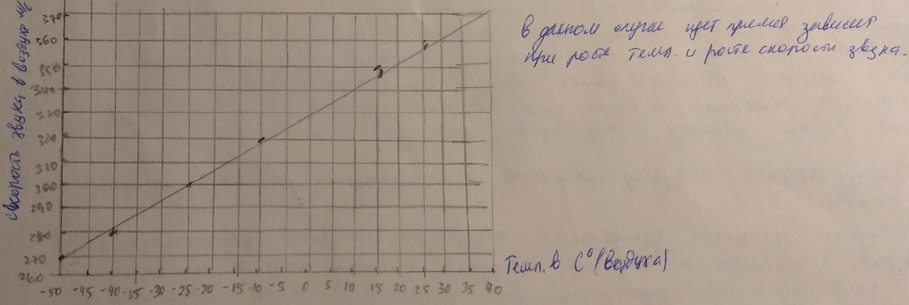
\includegraphics[width = 1\linewidth]{g}
	
	\item Что такое степени свободы молекул газа? Как вычисляются полные степени свободы молекул газа с учётом поступательных, вращательных и колебательных степеней свободы молекул? Расчитайте полное число свободы для О$ _2 $ и СО$ _2 $ с учетом и без колебательных степеней свободы.
	
	В классической механике молекула
	двухатомного газа в первом приближении рассматривается как совокупность
	двух материальных точек, жестко связанных недеформируемой связью. Эта система кроме трех степеней
	свободы поступательного движения имеет еще две степени свободы вращательного движения. Вращение вокруг третьей оси (оси, проходящей через оба атома) лишено смысла. Таким образом,
	двухатомный газ ($O_2$) обладает пятью степенями свободы ($i = 5$).
	Трехатомная ($CO_2$) и многоатомная нелинейные молекулы имеют
	шесть степеней свободы: три поступательных и три вращательных($i = 6$). Естественно, что жесткой связи между атомами не существует. Поэтому для реальных молекул необходимо учитывать
	также степени свободы колебательного движения.
	
	С учётом колебательных степеней свободы:
	
	$i = i_{v} + i_{r} + 2i_{N}$
	
	$i_N = 3N - 6$
	
	Для ($O_2$)  $i = 6$.
	
	Для ($CO_2$) $i = 9$.
	
	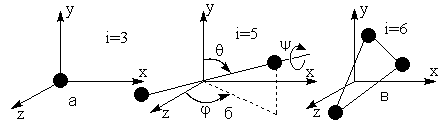
\includegraphics[width = 1\linewidth]{mol}
	
	
	\item Какие процессы политропные? Как вычисляется теплоёмкомть политропного процесса?
	
	Политропный процесс --- термодинамический процесс, во время которого удельная теплоёмкость газа остаётся неизменной. 
	
	Так как политропный процесс имеет постоянную теплоёмкость, показатель $ n $ может быть расчитан как $ \dfrac{C-C_p}{C-C_v} $.
	
	Где $ C_v = \dfrac{iR}{2} $ и $ C_p = \dfrac{(i+2)R}{2} $.
	
	Теплоёмкость политропического процесса
	
	\begin{equation}
		C = C_V\dfrac{n - \gamma}{n - 1}
	\end{equation}
	
	
	\item Какой процесс адиабатный? Что такое показатель адиабаты и чему он равен при двухатомном газе?
	
	Если сжатие и растяжение газа проискодит быстро, то области сжатия и растяжения не успевают обмениваться теплом, это описывает адиабатический процесс. Его показатель $ \gamma = \dfrac{C_p}{C_v} $, равен отношению теплоёмкости газа и изобарном и изохорном процессах. При двухатомном газе, где степень свободы 5, $ \gamma = 1.4 $.
	
	\item Как связаны между собой мольные и удельные теплоёмкости в изобарном и изохорном процессах? Как они вычисляются?
	
	Количество теплоты, необходимое для нагревания единицы массы вещества на 1 градус называется удельной теплоёмеостью.
	
	Для измерения удельной теплоёмкости газов используют молярную теплоёмкость, где единицой вещества является моль:
	
	\begin{equation}
	C_\mu = C\mu
	\end{equation}
	
	Уравнение Майера
	
	\begin{equation}
	C_p = C_v + R
	\end{equation}
	
	Формула Майера для удельной теплоёмкости:
	
	\begin{equation}
	\dfrac{C_p}{\mu} = \dfrac{C_v}{\mu} = \dfrac{R}{\mu}
	\end{equation}
	
	
\end{enumerate}

 


\end{document}